\section{Datenhaltung}

\subsection{Datenbank}
Die Daten des Web-Service werden in einer Datenbank und in Ordnern organisiert. 
Nutzerdaten und Videodaten werden in Tabellen gespeichert. Als Syntax wird PostgreSQL verwendet. 

\begin{figure}[ht]
	\centering
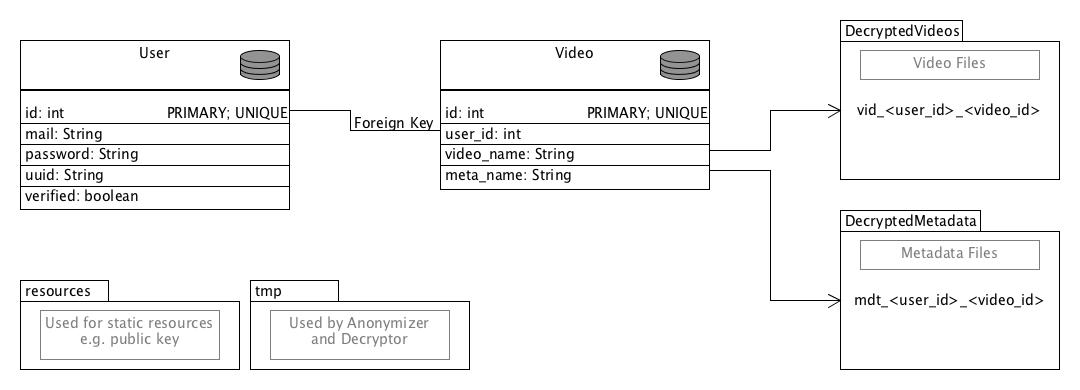
\includegraphics[width=1\textwidth]{./resources/Diagramme/Webservice/database_scheme.jpg}
\caption{Datenbankschema}
	\label{fig:overview_mvp}
\end{figure}

Die User-Tabelle für die Nutzerdaten speichert eine einzigartige Nutzer-Id, die Email-Adresse, das Passwort und ob der Nutzer bereits seinen Account verifiziert hat.\newline
Die Video-Tabelle für Videodaten speichert eine einzigartige  Video-Id, die Nutzer-Id des Nutzers, der das Video hochgeladen hat sowie den Videodateiname und den Metadatendateiname. die Nutzer-Id agiert hier als Fremdschlüssel, die Dateinamen werden zum referenizieren der Dateien aus den Ordnern verwendet.\newline
Video und Metadaten werden in jeweils einem eigenen Ordner organisiert. Dabei teilen sich Videodateien aller Nutzer einen Ordner und Metadatendateien aller Nutzer einen Ordner. Der Dateiname wird stets aus einem statischen Anfang und der Kombination aus Nutzer-Id und Video-Id zusammengesetzt und ist daher einzigartig.\newline
Darüber hinaus existiert noch ein weiterer Ordner namens \textit{tmp}, welcher von Anonymizer und Decryptor verwendet wird und in den tmporär Dateien abgespeichert werden. Es existieren keine Schnittstellen um von außen direkt auf Inhalte dieses Ordners zuzugreifen.

\subsection{Temporäre Dateien}
Die Verwaltung der temporären Dateien für die Bearbeitung der Videos übernimmt das \nameref{service:modul:VideoProcessing} Modul. Dies ist notwendig, da die entstehenden und benötigten Daten ausschließlich abhängig von den Arbeitsschritten der \nameref{service:klasse:VideoProcessingChain} ist und daher nicht von anderen Modulen des Web-Dienstes beeinflusst werden soll. Der Web-Dienst stellt dafür den \textit{tmp} Ordner bereit.\newline
Der \nameref{service:klasse:EditingContext} erzeugt dann alle für die Bearbeitung notwendigen Dateipfade in der Form:\newline
benutzername\_videoname\_attribut.endung

\subsection{Verwendete Resourcen}
Für die Bearbeitung der Videos verwendete Resourcen (z.B. der private Key des \nameref{service:klasse:RSADecryptor} oder der CascadeClassifier des \nameref{service:klasse:ExampleAnalyzer}) werden im "'resources"' Ordner abgelegt.
